\titleformat {\chapter} {\normalfont\huge\bfseries\color{black}}   {\thechapter}{10pt}{\huge} 
\chapter {Related Research Work}

%% ================================
%% \input{Advice-on-Chapter-4}
%% ================================
	
\section{UMP CNC Research machine}\label{sec:4.1-CNC-Research-Machine}

The images of the UMP 3-axis CNC research machine for our previous work are provided in next three figures. It is an experimental CNC router-type, that instead of a tool cutter, uses a pen to create drawings on paper in the X-Y plane. The Z-axis motion is used to raise and lower the pen. As a consequence, circular arc (G02, G03 G-Code) moves are applicable to the X and Y axes only, while linear (G01 G-Code) moves are applicable to all three X, Y and Z axes.  
\vspace*{1\baselineskip}
		
The CNC Research machine is driven on each axis by the Panasonic Minas A4, alternating current (AC) servo system. The configuration for each axis consists of a servo-driver and a servo-motor pair. Each servo-motor is installed on a ball-screw shaft. Electrical TTL-type, 0 to 5 volts, digital pulses are used as input signals to drive the servo-driver. Since each motor is installed on a ball-screw shaft, the motor rotational motion gets converted to linear translational motion in the direction of each axis. 
\vspace*{1\baselineskip}

\begin{figure}[htbp]
\begin{center}
	\frame{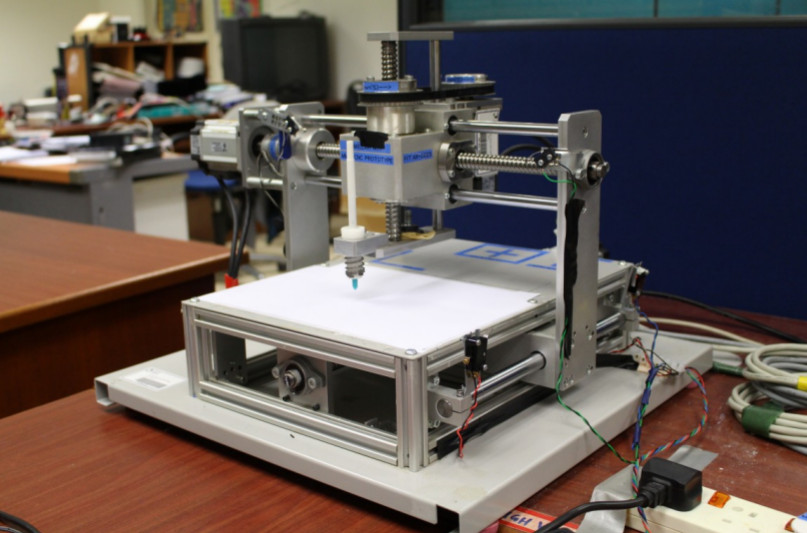
\includegraphics[width=0.85\textwidth]{./07-images/img-Ch4/CNC-Research-Machine-3-Axis.jpg}}
	\caption{The UMP 3-axis CNC Research Machine}
	\label{fig:CNC-Research-Machine-3-Axis.jpg}
\end{center}
\end{figure}

Electrical signal pulses sent to the servo-driver provide information like rotate clockwise (CW), rotate counter-clockwise(CCW), travel distance to rotate, speed to rotate, and so on. The actuation using electrical pulses makes the physical CNC machine instantaneously active. 

% =====================================================
\clearpage
\pagebreak

\begin{figure}[htbp]
	\begin{center}
		\frame{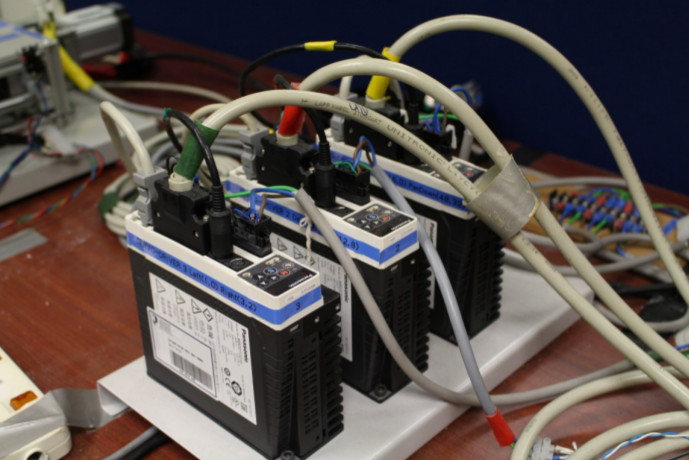
\includegraphics[width=0.73\textwidth]{./07-images/img-Ch4/CNC-Research-Machine-3-Sets-Servo-Drives.jpg}}
		\caption{Servo-Drives for the 3-Axis CNC Research Machine}
		\label{fig:CNC-Research-Machine-3-Sets-Servo-Drives.jpg}
	\end{center}
\end{figure}

\begin{figure}[htbp]
	\begin{center}
		\frame{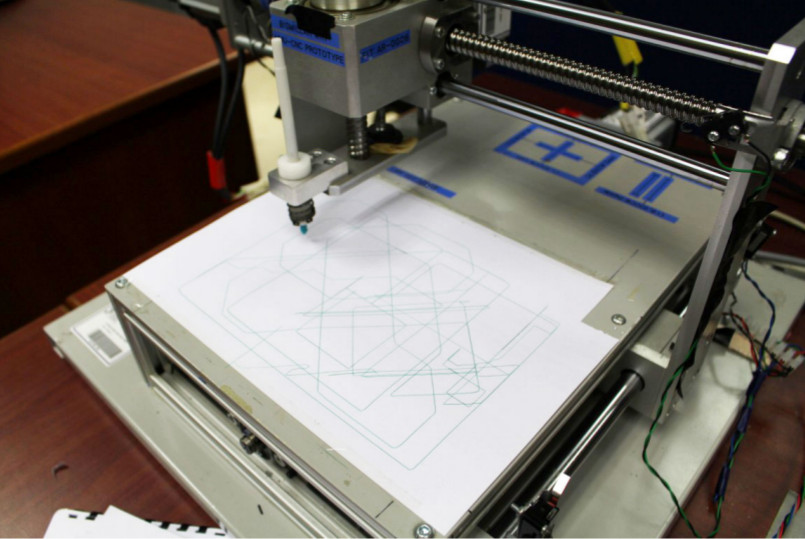
\includegraphics[width=0.73\textwidth]{./07-images/img-Ch4/CNC-Research-Machine-X-Y-Movements.jpg}}
		\caption{CNC Research Machine X-Y Movements}
		\label{fig:CNC-Research-Machine-X-Y-Movements.jpg}
	\end{center}
\end{figure}


For our CNC research machine, we used a commercial, industry standard, Panasonic MINAS A4 AC servo-driver and servo-motor pair. We have three sets of this pair because the research machine is a 3-axis CNC servo driven machine. 
\vspace*{1\baselineskip}

Each Panasonic MINAS A4 servo-motor is a 24-volts, 750-watts, high torque, alternating current (AC) driven motor. It can be configured to operate in a single-phase or a three-phase, AC 60 Hz input current mode.
\vspace*{2\baselineskip}\\

We can configure our CNC research machine to run in three control modes: position control, velocity control, and torque control. It can also be configured either in an open-loop or a closed-loop control scheme.  
\vspace*{1\baselineskip}

The CNC research machine was procured on a joint collaboration project between University Malaysia Pahang (UMP) and Multimedia University, Cyberjaya (MMU), in the year 2008, under the E-Science grant, Ministry of Science, Technology and Environment (MOSTE), Government of Malaysia.  

% =======================
% \clearpage
% \pagebreak

\section{Previous CNC research projects}

We have successfully developed and executed C/C++ software codes using various devices to drive our CNC research machine. We have written codes that combine the following programming techniques: standard serial-running codes, realtime-running codes (RTAI) and parallel-running codes.  
\vspace*{1\baselineskip}

All of the pulse-generator devices that we have used on all of our research projects run C/C++ software codes on the open source Linux platform. On Linux, every software that we need is cost-free and open source. The C/C++ software compiler is cost-free. We even customize the operating system kernel to meet our needs. All of the interpolation computations we accomplished in our projects are of reference-pulse CNC interpolations. 
\vspace*{1\baselineskip}

We avoided the Microsoft (MS) Windows platform because we need full and open access to the operating system and to the software components that control the devices attached to the operating system. In addition, Microsoft Windows operating system is not free. Even, the C/C++ software compiler is not cost-free. In many cases, we cannot find suitable software applications on MS Windows that meets our project needs and that are cost-free. For low-level systems programming (our type of projects), the MS Windows is not a suitable platform for a cost-free development environment.  
% \vspace*{1\baselineskip}

\section{Previous software programming experiences}

On programming experience, we covered realtime execution using RTAI kernel modules on the LinuxCNC system. In the Raspberry Pi 3 project, we managed to drive the CNC system using C++ multi-threading. The concept of RTAI interrupt-style programming architecture can be found in the appendix at [\ref{fig:App4-rtai-architecture-on-linux.jpg}]. 
\vspace*{1\baselineskip}

Examples of realtime codes that we have used in our projects can be found in the appendix at [\ref{App4-Summary main() function C-Code listing for RTAI}], [\ref{App4-Full C-Code listing for Real Time (RTAI)}], and [\ref{App4-Full execution C/C++ code for Real Time (RTAI)}].  
\vspace*{1\baselineskip}

Examples of parallel C/C++-2011 codes using multi-threading can be found in the appendix at [\ref{App4-C++2011 Example Parallel Multithreading}] and [\ref{App4-C++2011 Execution Parallel Multithreading}], while codes for parallel C/C++ MPI (Message Passing Interface) using multi-processing can be found in the appendix at [\ref{App4-C++-MPI Example Parallel Multiprocessing}] and [\ref{App4-C++-MPI Execution Parallel Multiprocessing}]. 
\vspace*{1\baselineskip}

For our research project, we will combine both realtime and parallel codes suitably to meet our CNC machine needs. We will also consider integrating codes or taking ideas from modern and efficient computer programming languages like \href{https://www.rust-lang.org/}{Rust programming language}, with an example multithreading code at [\ref{App4-Rust Parallel Multithreading Codes}] placed in the appendix. Rust is an upcoming low level systems language, a direct competitor to C/C++. Rust was designed from the ground up with Safety, Security and Concurrency (SSC) built-into the Rust engine. This is unlike the C/C++ language or most languages, where these functionality come as separate linked software libraries. More will be discussed in the section on literature review.
\vspace*{1\baselineskip}

Internally, inside the CNC control software we may use \href{https://www.python.org/}{Python programming language} or \href{https://julialang.org/}{Julia programming language} scripts, that have excellent processing and data handling capabilities. These languages support parallel programming internally not through external libraries. This researcher is quite well versed in the use of these computer programming languages. Example codes for Python multithreading and multiprocessing can be found in the appendix at [\ref{App4-Python Parallel Multithreading}] and [\ref{App4-Python Parallel Multithreading}]. And similarly, parallel codes for the Julia language are provided in the appendix at [\ref{App4-Julia Parallel Programming Codes}].
\vspace*{1\baselineskip}

The CNC machine only needs electrical pulses of the right characteristics to run. The kind of devices that generate these electrical pulses does not matter. However, the interface software codes varies between different hardware devices.  
\vspace*{1\baselineskip}

As an example, the full C/C++ software codes that actually generate electrical pulses at the serial and parallel ports of the computer concurrently, is provided in the appendix at this link, [\ref{sec:App4-Write-Parallel-Serial-Ports}]. The named, Concurrent-Writes-to-Parallel-and-Serial-Ports program, is the boundary point (or transition point) where "software codes write bits that finally generate hardware electrical pulses". This bit-writing software program is essentially the CNC Signal Driver software, that in turn takes inputs from the CNC Signal File. The CNC Signal File is, in turn, the output of the complicated work executed by the CNC Interpreter and CNC Interpolator combination, that also in turn, takes its inputs from the G-Code file, which is the starting point of the entire CNC operations. 
\vspace*{1\baselineskip}

Essentially, what we have described above is the "software backward trail" to its starting point in CNC machine operations. From the clarification above, we realize that in order to accomplish this project successfully, from start to finish, software design knowledge, software programming methods and software implementation skills are evidently important.

% \vspace*{1\baselineskip}
% ====================================
% \clearpage
% \pagebreak
\section{Pulse generator devices}

\subsection{Computer extension boards}
The following are projects we have undertaken using pulse generator devices that successfully drive the CNC research machine. For computer extension boards as pulse generator devices, we worked on the following six(6) devices for our research: 
\begin{enumerate}
	\item PC parallel port, [\ref{fig:App4-Captured-Parallel-Port-Built-in-Motherboard.jpg}], [\ref{fig:App4-Captured-Parallel-Port-PCI-Adapter-Card.jpg}], [\ref{fig:App4-Captured-USB-to-Parallel-Port-PL2305-Converter.jpg}].
	
	\item Velleman K8000 Parallel extension board, [\ref{fig:App4-Captured-Velleman-K8000 Parallel-Port-Extension-Board.jpg}].
	
	\item Velleman K8055 USB extension board, [\ref{fig:App4-Captured-Velleman-K8055-USB-Extension-Board.jpg}].
	
	\item Heber X10i USB extension board, [\ref{fig:App4-Captured-Heber-X10i-USB-Extension-Board.jpg}].
	
	\item Arduino Due USB extension board, [\ref{fig:App4-Captured-Arduino-Due-USB-Extension-Board.jpg}].
	
	\item Digilent Nexys-3 Spartan-6 FPGA board. [\ref{fig:App4-Captured-Nexys3-Spartan6-FPGA-USB-Extension-Board.jpg}].
	
\end{enumerate}
 
% \vspace*{1\baselineskip}

\subsection{Single Board Computers}

For single board computers (SBC) as pulse generator devices, we worked on the following three(3) systems for our research: 
\begin{enumerate}
	\item Raspberry Pi SBC, General purpose. [\ref{fig:App4-Captured-Raspberry-Pi3-ModelB-SBC.jpg}], [\ref{fig:App4-Captured-Raspberry-Pi2-ModelB-SBC.jpg}].
	
	\item Banana Pi SBC, Graphic processing focus. [\ref{fig:App4-Banana-PI-M2U-SBC.jpg}].
	
	\item Beagle-Board xM SBC. Graphic processing plus DSP focus. [\ref{fig:App4-Beagle-Board-xM-SBC.jpg}].
	
\end{enumerate}

The above three(3) SBCs all have different brands of processors (CPUs). The Raspberry Pi SBC hardware is suited for general purpose use, while the Banana Pi SBC and BeagleBoard xM SBC are graphic processing focused.
\vspace*{1\baselineskip}

In addition, we have chosen to study Beagle-Board xM  because it has a digital signal processor (DSP) chip, which is not available on both the Raspberry Pi SBC or the Banana Pi SBC.
\vspace*{1\baselineskip}

The primary purpose of all nine(9) devices mentioned above, is to generate electrical pulses through the associated pins on each board. Writing software that generates pulses (high/low for 1/0) at the pins means binary representation in software terms. This is another critical software programming activity in CNC development. 
\vspace*{1\baselineskip}

We need to write software that converts codes into binary formatted strings, for example, generating 8-bit binary strings to drive eight(8) individual parallel lines simultaneously, parallel in time. Similarly, with 16-bit binary strings, we can drive 16 parallel lines simultaneously. Fot that purpose, we provided the full C/C++ program code that converts outputs to 8-bit, 16-bit, and 32-bit binary strings in the appendix at  [\ref{App4-Converting-software-codes-to-binary-bits-pulses}]. 
\vspace*{1\baselineskip}

Even though the binary string generation is common, the actual software driving implementation varies between boards. This arises due to the different pin configurations on each hardware device. We succeeded in our previous projects by manipulating software codes for each board, accordingly.

% \pagebreak
\section{Computer Extension Boards as devices}

\subsection{Project 1 - PC parallel port}

The parallel port hardware in a computer can be a built-in device located on the mother-board or an add-in PCI card attached to the PCI bus of the mother-board. 
\vspace*{1\baselineskip}

There are also converter devices, that converts USB to parallel port, like the Profilic USB to IEEE1284 Bridge Controller Bi-Direction Parallel Interface that uses the PL2305 software driver and is supported on both Windows and Linux. The parallel port software driver must be installed on the Linux computer for software to communicate with it. 
\vspace*{1\baselineskip}

A parallel port control program code written in C/C++ provides commands for the parallel port device (hardware) to generate electrical pulses to drive the CNC machine. The parallel port pins are appropriately connected (wired electrically) to the different servo-drivers of the CNC machine.
\vspace*{1\baselineskip}

The report for this work is at reference \cite{FYP_Abzal_2012}. In this scheme, the various devices connected to the Linux computer are the devices responsible for generating electrical pulses that drives the CNC machine. Images of the parallel port devices that we have used are provided at [\ref{fig:App4-Captured-Parallel-Port-Built-in-Motherboard.jpg}] for parallel port built-in the computer motherboard,  [\ref{fig:App4-Captured-Parallel-Port-PCI-Adapter-Card.jpg}] for the parallel port PCI adapter card and [\ref{fig:App4-Captured-USB-to-Parallel-Port-PL2305-Converter.jpg}] for the USB-to-Parallel port PL2305 converter cable.


\subsection{Project 2 - Velleman K8000 Parallel extension board}

The Velleman K8000 is a computer interface board, a hardware card to control external electrical devices with our computer through the standard parallel cable. The card offers some analog/digital connections to do this.
\vspace*{1\baselineskip}
	
The card is provided with software drivers to run on both Windows and Linux computers. For the K8000 board, software programs on the computer can directly communicate via the parallel protocol IEEE1284 with the board. Software codes can be written in different programming languages like C/C++, Python, VB, Qbasic and Turbo Pascal. 
\vspace*{1\baselineskip}
	
Similarly, a parallel port control program code written in C/C++ provides commands for the parallel port device (hardware) to generate electrical pulses to drive the CNC machine. 
\vspace*{1\baselineskip}
	
The K8000 board digital output pins are appropriately connected (wired electrically) to the different servo-drivers of the CNC machine. On the Velleman K8000 board, the electrical pulses can be seen during CNC execution because LEDs (blinking on and off) are provided for selected pins.
\vspace*{1\baselineskip}

The report for this work is at reference \cite{FYP_Abzal_2012}.	In this scheme, the Velleman K8000 Parallel interface board hardware is the device responsible for generating electrical pulses that drives the CNC machine. The image of the K8000 parallel interface board that we have used is provided at [\ref{fig:App4-Captured-Velleman-K8000 Parallel-Port-Extension-Board.jpg}].

\subsection{Project 3 - Velleman K8055 USB extension board}

The Velleman K8055 board is a USB extension board that has 5 digital input channels and 8 digital output channels. There are two analogue inputs and two analogue outputs with 8 bit resolution. The number of inputs and outputs can be further expanded by connecting up to a maximum of four K8055 cards. 
\vspace*{1\baselineskip}

The board is provided with software drivers to run on both Windows and Linux computers. For the K8055 board, software programs on the computer can directly communicate via the USB protocol with the board. It is like driving a typical USB printer. Software codes can be written in different programming languages like C/C++, Delphi, Python, Visual Basic, Qbasic and Turbo Pascal.
\vspace*{1\baselineskip}

Similarly, a USB port control program code written in C/C++ provides commands for the USB port device (hardware) to generate electrical pulses to drive the CNC machine. The K8055 board digital output pins are appropriately connected (wired electrically) to the different servo-drivers of the CNC machine. Also on the Velleman K8055 board, the electrical pulses can be seen during CNC execution because LEDs (blinking on and off) are provided for selected pins.
\vspace*{1\baselineskip}

The report for this work is at reference \cite{FYP_Rajeef_2015}. In this scheme, the Velleman K8055 USB interface board hardware is the device responsible for generating electrical pulses that drives the CNC machine. The image of the K8055 USB interface board that we have used is provided at [\ref{fig:App4-Captured-Velleman-K8055-USB-Extension-Board.jpg}]. 

\subsection{Project 4 - Heber X10i USB extension board}

The Heber X10i USB Board is also an extension board connected to the Linux computer via the USB port. The Heber X10i software driver must be installed on the Linux computer for software to communicate with it. The Heber board digital output pins are connected (wired electrically) to appropriate servo-drivers for the 3-axis CNC machine. 
\vspace*{1\baselineskip}

For the Herber board, software programs written in C/C++ on the Linux machine can directly communicate via USB with the board. It is like driving a typical USB printer. 
\vspace*{1\baselineskip}

As an extension board, there is no need for a compiled firmware to be downloaded onto the Heber board. Software instructions to generate electrical pulses come directly from the C/C++software programs on the Linux computer. Software codes can be written in different programming languages like C/C++ and Python.
\vspace*{1\baselineskip}

The report for this work is at reference \cite{FYP_Saleh_2014}. In this scheme, the Heber X10i USB Board is the device responsible for generating electrical pulses. The image of the  Heber X10i USB board that we have used is provided at [\ref{fig:App4-Captured-Heber-X10i-USB-Extension-Board.jpg}].


\subsection{Project 5 - Arduino Due USB extension board}

The Arduino Due board is an extension board connected to the Linux computer via the USB port. The Arduino Due software driver must be installed on the Linux computer for software to communicate with it. 
\vspace*{1\baselineskip}

A control program written in C/C++ on the Linux machine is compiled to produce machine codes (basically firmware) that is downloaded and installed into the memory of the Arduino Due board. 
\vspace*{1\baselineskip}

For the Arduino Due board, software programs on the computer cannot directly communicate online with the board. When any changes made in the software code to drive the CNC machine, it has to be recompiled and re-downloaded to the Arduino Due memory. This is different from the driving schemes in both Velleman K8000, Velleman K8055 and Heber X10i boards, where control programs on the Linux machine can directly drive electrical pulses through the boards to the CNC machine. 
\vspace*{1\baselineskip}

The relevant digital output pins on the Arduino Due are appropriately connected (wired electrically) to the CNC machine. 
\vspace*{1\baselineskip}

The report for this work is at reference \cite{FYP_Hazmi_2014}. In this scheme, the Arduino Due USB Board is the device responsible for generating electrical pulses. The image of the  Arduino Due USB board that we have used is provided at [\ref{fig:App4-Captured-Arduino-Due-USB-Extension-Board.jpg}].

% \pagebreak
\subsection{Project 6 - Digilent Nexys-3 Spartan-6 FPGA USB board}

The FPGA (Field Programmable Gate Array) USB board is also an extension board connected to the Linux computer via the USB port. The FPGA board software driver must be installed on the Linux computer for software to communicate with it.
\vspace*{1\baselineskip}

FPGAs are semiconductor devices comprising programmable logic blocks and interconnection circuits. It can be programmed or re-programmed to the required functionality after manufacturing. Programming FPGA generates firmware. It was said that FPGA is about using software to program hardware.
\vspace*{1\baselineskip}

The FPGA firmware for the Nexys-3 Spartan-6 FPGA, is a compiled VHSIC Hardware Description Language (VHDL) software on the Linux computer. After compilation it is downloaded onto the FPGA board to control the board. 
\vspace*{1\baselineskip}

The FPGA board digital output pins are connected with wires to appropriate servo-drivers for the 3-axis CNC machine. 
\vspace*{1\baselineskip}

After installation of the firmware on the FPGA board, software program instructions written in C/C++ on the Linux machine can directly communicate via USB with the board. With these received instructions, the FPGA pins appropriately generate the required electrical pulses to the CNC machine. 
\vspace*{1\baselineskip}

The Nexys-3 FPGA hardware development board manufactured by Digilent Inc. This board was used to control the CNC machine using its programmable input/output (I/O) pins. This hardware is a USB extension board to the Linux computer. The board was installed with a set of software drivers for the Linux platform.
\vspace*{1\baselineskip}

A linux based personal computer running Ubuntu 10.04 LTS (Long Term Support) with RTAI (Real Time Application Interface) was deployed. The linux kernel version was linux-2.6.32-122-rtai, and was installed as part of the LinuxCNC system.   
\vspace*{1\baselineskip}

The FPGA board is an external control board connected to the linux computer via a USB port. The FPGA board pins were then connected with wires to appropriate servo-drivers for the 3-axis CNC machine. 
\vspace*{1\baselineskip}

The Xilinx ISE ver. 14.7 software application was used to generate the FPGA firmware. The FPGA firmware program was written using VHSIC Hardware Description Language (VHDL) language. VHDL is a hardware description language used in electronic design automation to describe digital and mixed-signal systems such as field-programmable gate arrays (FPGA) and integrated circuits (ICs). 
\vspace*{1\baselineskip}

VHDL is hardware programming using software, that results in firmware. Firmware is loaded into hardware to make the hardware work, basically controls the hardware. VHDL is inherently a general purpose parallel programming language. A VDHL program source code was created on the personal computer. The Xilinx ISE application compiles this VDHL code into a firmware code we called (FPGA-NEXYS3). This generated firmware was then uploaded from the computer into the FPGA board. Now the board is ready for use with our CNC machine. 
\vspace*{1\baselineskip}

Essentially, the VHDL programming that was carried out to produce the FPGA-NEXYS3 firmware code is to map FPGA parameters and hardware pins for connections to servo-drivers for the 3-axis CNC machine. The G-Code File Interpreter (GFI) software was developed on the Linux platform. The Signals File Sender (SFS) software was developed on the Linux platform using C/C++ code. 
\vspace*{1\baselineskip}

It is important to note that in this FPGA research project, it is the combination of three(3) components: the GFI, the SFS and the FPGA-NESYS3 firmware that drive the CNC machine. First, a RS274D NGC G-Code file is processed by the GFI program to produce a signals file. Next, the SFS program transmits the contents of this signals file to the FPGA board. 
\vspace*{1\baselineskip}

The FPGA board with ready loaded-to-use FPGS-NEXYS3 firmware automatically sends separate electronic signals (pulses) in parallel to the individual servo-drives of the 3-axis CNC machine.
\vspace*{1\baselineskip}

The report for this work is at reference \cite{FYP_Charles_2014}. In this scheme, the Nexys-3 Spartan-6 FPGA USB Board is the device responsible for generating electrical pulses to drive the CNC machine. The image of the  FPGA USB board that we have used is provided at [\ref{fig:App4-Captured-Nexys3-Spartan6-FPGA-USB-Extension-Board.jpg}].

% ==========================================
% \clearpage
% \pagebreak

\section{Single Board Computers as devices}

\subsection{Project 7 - Raspberry Pi 2 and Raspberry Pi 3 SBC boards}

The Raspberry Pi 3 Model B, is a cheap, tiny credit card size, full-fledged computer system that can run software applications. It is called a Single Board Computer (SBC). The Raspberry Pi 2 is similar to Raspberry Pi 3, but is has less memory, less CPU speed (GHz), less USB ports, and less in everything. However, it works the same. This SBC is based on the ARM CPU processor and not the Intel CPU processor. This SBC includes built LAN and wireless networking. 
\vspace*{1\baselineskip}

The SBC (single board computer) is a true full-fledged computer in itself. It is not an extension board to some computer. The SBC is like a "desktop" computer that requires external peripherals. To use this Raspberry Pi SBC, we need just connect a keyboard, mouse, display monitor, power supply, and a micro SD card with an installed Linux Distribution, in a manner similar to connecting the same peripherals to the desktop computer. 
\vspace*{1\baselineskip}

With an operating system like Raspbian (Ubuntu-based) installed, we have full fledged Linux capabilities on the Raspberry Pi, including all software applications and language compilers available for Linux Ubuntu. The required software drivers, for example, BCM2835 must be installed to access specified components and peripherals on the Raspberry Pi.
\vspace*{1\baselineskip}

The Raspberry Pi digital output pins are connected with wires directly to appropriate servo-drivers for the 3-axis CNC machine. Software programs written in C/C++, residing on the Raspberry Pi can directly drive electrical pulses through the digital output pins to the CNC machine. There is no need for any other computer.
\vspace*{1\baselineskip}

The report for this work is at reference \cite{FYP_Asyrul_2017}. In this scheme, the Raspberry Pi-3 Model-B SBC is the device responsible for generating electrical pulses to drive the CNC machine. 
\vspace*{1\baselineskip}

The image of the  Raspberry Pi-3 Model-B that we have used is provided at [\ref{fig:App4-Captured-Raspberry-Pi3-ModelB-SBC.jpg}] and for the Raspberry Pi-2 Model-B is provided at [\ref{fig:App4-Captured-Raspberry-Pi2-ModelB-SBC.jpg}]. The image comparison between Raspberry Pi-3 and Raspberry Pi-2 is provided at [\ref{fig:App4-Captured-Raspberry-Pi2-ModelB-SBC.jpg}].
% \vspace*{1\baselineskip}

\subsection{Project 8 - Banana Pi BPI-M2 SBC board}

Banana Pi BPI-M2 Ultra is a quad-core mini single board computer built with Allwinner R40 SoC. It features 2GB of RAM and 8GB eMMC. It also has onboard WiFi and BT. On the ports side, the BPI-M2 Ultra has 2 USB A 2.0 ports, 1 USB OTG port, 1 HDMI port, 1 audio jack, a DC power port, and last but not least, a SATA port.
\vspace*{1\baselineskip}

Also being a member of the Banana Pi family, the M2 Ultra is a direct upgrade from the Banana Pi M1/M1+ that support SATA from the SoC. The SATA performance on the R40 is fitting for media related projects such as storage servers. Backed by our community, starting a project and building servers is fun and rewarding. 
\vspace*{1\baselineskip}

The Banana Pi operating system is similar to the Raspberry Pi, but a modified version to suit its hardware. It uses the same Raspbian system based on the Ubuntu software for desktops and notebooks. Software C/C++ programming is the same as for the Raspberry Pi. The only difference is the software driver for devices on the board. Raspberry Pi uses different hardware chips on its board compared to the Banana Pi, basically their product differentiations and marketing strategy.  
\vspace*{1\baselineskip}

The report for this work is at reference \cite{FYP_Rajeef_2015}. In this scheme, the Banana Pi BPI-M2 SBC is the device responsible for generating electrical pulses to drive the CNC machine. The image of the Banana Pi BPI-M2 SBC that we have used is provided at [\ref{fig:App4-Banana-PI-M2U-SBC.jpg}].

\subsection{Project 9 - Beagle-Board xM SBC board}

The BeagleBoard is a pocket-sized reference board containing a Texas Instruments Open Multimedia Application Platform (OMAP) 3 system-on-a-chip (SoC) processor, which includes an ARM Cortex-A8 core, Texas Instruments C64x+ digital signal processor (DSP), and onboard graphics engine, as well as integrated dual data rate (DDR) random-access memory (RAM). The BeagleBoard is an inexpensive platform for hobbyists, academics, and professionals who are learning Linux and small systems.
\vspace*{1\baselineskip}

We chose this BeagleBoard xM for research because it has a digital signal processor (DSP), which is not available on the Raspberry Pi SBC or the Banana Pi SBC.
\vspace*{1\baselineskip}

Similarly, the Beagle-Board xM operating system is similar to the Raspberry Pi, but a modified version to suit its hardware. It uses the same Raspbian system based on the Ubuntu software for desktops and notebooks. Software C/C++ programming is the same as for the Raspberry Pi. The only difference is the software driver for devices on the board. Raspberry Pi uses different hardware chips on its board compared to the Beagle-Board xM, basically their product differentiations and marketing strategy.  The report for this work is at reference \cite{FYP_Rajeef_2015}. In this scheme, the Beagle-Board xM SBC is the device responsible for generating electrical pulses to drive the CNC machine. The image of the Beagle-Board xM SBC that we have used is provided at [\ref{fig:App4-Beagle-Board-xM-SBC.jpg}].

\pagebreak
%% =========================================================
\section{Summary on Related Research Work}
%% =========================================================

We started by providing a brief description of our UMP CNC Research machine, a 3-axis experimental CNC router-type machine, that instead of using a tool cutter, uses a pen to create drawings on paper in the X-Y plane. We also showed images of the CNC Research machine. Each axis of the machine is driven by an alternating current servo-driver and servo-motor pair. The servo-driver can be driven using 3 different control strategies: position control, velocity control and torque control.
\vspace*{1\baselineskip}

Next, we mentioned that only C/C++ software codes were used on various hardware devices as pulse generators to drive the CNC Research machine. The written codes include combinations of standard serial-running codes, realtime-running codes (RTAI) and parallel multi-threaded running codes.  
\vspace*{1\baselineskip}

We ran the C/C++ software codes on the open source Linux platform only. We avoided the Microsoft (MS) Windows platform because it is not possible to get full and open access to the operating system environment, that is, to the hardware devices attached to the operating system. We concluded that the MS Windows environment is not a suitable platform for our specific research project.  
\vspace*{1\baselineskip}

All of the interpolation computations we accomplished in our projects are of reference-pulse type CNC interpolations. We also implemented both non-realtime and realtime executions on the CNC Research machine.
\vspace*{1\baselineskip}

Since the CNC machine only needs electrical pulses of the right characteristics to run, the kind of devices that generate these electrical pulses does not matter. On this matter, we described the hardware pulse generator devices comprising of six(6) computer extension board devices and three(3) single board computers (SBC) that we have successfully implemented in driving the CNC Research machine.
\vspace*{1\baselineskip}

For driving the CNC Research machine using the parallel port, the four(4) devices used comprised, the built-in parallel port on the computer motherboard, the parallel port PCI adapter card, the USB-to-Parallel port PL2305 converter cable and the Velleman K8000 Parallel extension board.
\vspace*{1\baselineskip}

For driving the CNC Research machine using the USB port, the four(4) devices used comprised, the Velleman K8055 USB extension board, the Heber X10i USB extension board, the Arduino Due USB extension board, and the Digilent Nexys-3 Spartan-6 FPGA USB development board.
\vspace*{1\baselineskip}

For driving the CNC Research machine using standalone Single Board Computers (SBC), the four(4) devices used comprised, the Raspberry Pi 2 and Raspberry Pi 3 SBC boards, the Banana Pi BPI-M2 SBC board, and the Beagle-Board xM SBC board. 
\vspace*{1\baselineskip}

In the Appendix for Chapter-4 at this link [\ref{sec:App4-Related-Research-Work}], we included some results on our previous CNC research. Following that, we included images and specifications of the various hardware pulse generator devices we have successfully implemented on our CNC Research machine. And we included full contents of realtime and parallel running software codes, as examples.



% ==========================================================
